
\documentclass{article}

\usepackage[utf8]{inputenc}

\usepackage{amsmath, bm}
\usepackage{graphicx}
\usepackage{amssymb}
\usepackage{float}
\usepackage{caption}
\usepackage{subcaption}
\usepackage{hyperref}
\usepackage{tikz}
\usepackage{layout}

\usepackage[margin=1in]{geometry}
\usepackage{listings}
\usepackage{xcolor}
\usepackage{color, colortbl}
\usepackage{textgreek}
\usepackage{mathrsfs}
\usepackage{savetrees}

\usepackage{titlesec}

\titleformat{\subsubsection}
  {\normalfont\selectfont}{\thesubsubsection}{1em}{}

\usetikzlibrary{calc}
\usetikzlibrary{angles,quotes} % for pic
\usetikzlibrary{patterns,snakes}
\usetikzlibrary{arrows}
\tikzset{>=latex} % for LaTeX arrow head

\setlength{\parskip}{\baselineskip}%
\setlength{\parindent}{0pt}%
\linespread{0.9}


\definecolor{codegreen}{rgb}{0,0.6,0}
\definecolor{codegray}{rgb}{0.5,0.5,0.5}
\definecolor{codepurple}{rgb}{0.58,0,0.82}
\definecolor{backcolour}{rgb}{0.95,0.95,0.92}

\lstdefinestyle{mystyle}{
    backgroundcolor=\color{backcolour},   
    commentstyle=\color{codegreen},
    keywordstyle=\color{magenta},
    numberstyle=\tiny\color{codegray},
    stringstyle=\color{codepurple},
    basicstyle=\ttfamily\footnotesize,
    breakatwhitespace=false,         
    breaklines=true,                 
    captionpos=b,                    
    keepspaces=true,                 
    numbers=left,                    
    numbersep=5pt,                  
    showspaces=false,                
    showstringspaces=false,
    showtabs=false,                  
    tabsize=2
}

\lstset{style=mystyle}


\begin{document}

\title{}
\author{lwp26}
\date{November 2024}
\maketitle 

\iffalse
\begin{abstract}
    \centering
    LOg bAs
\end{abstract}
\fi

%-----------------------------------------------------------------------------------------
\section{Introduction}
%-----------------------------------------------------------------------------------------

\subsection{Objectives}

\subsection{Setup}

\section{LATERAL CREEP}

\subsection{\textbf{Transducer Calibration}}

\begin{figure}[H]
    \centering
    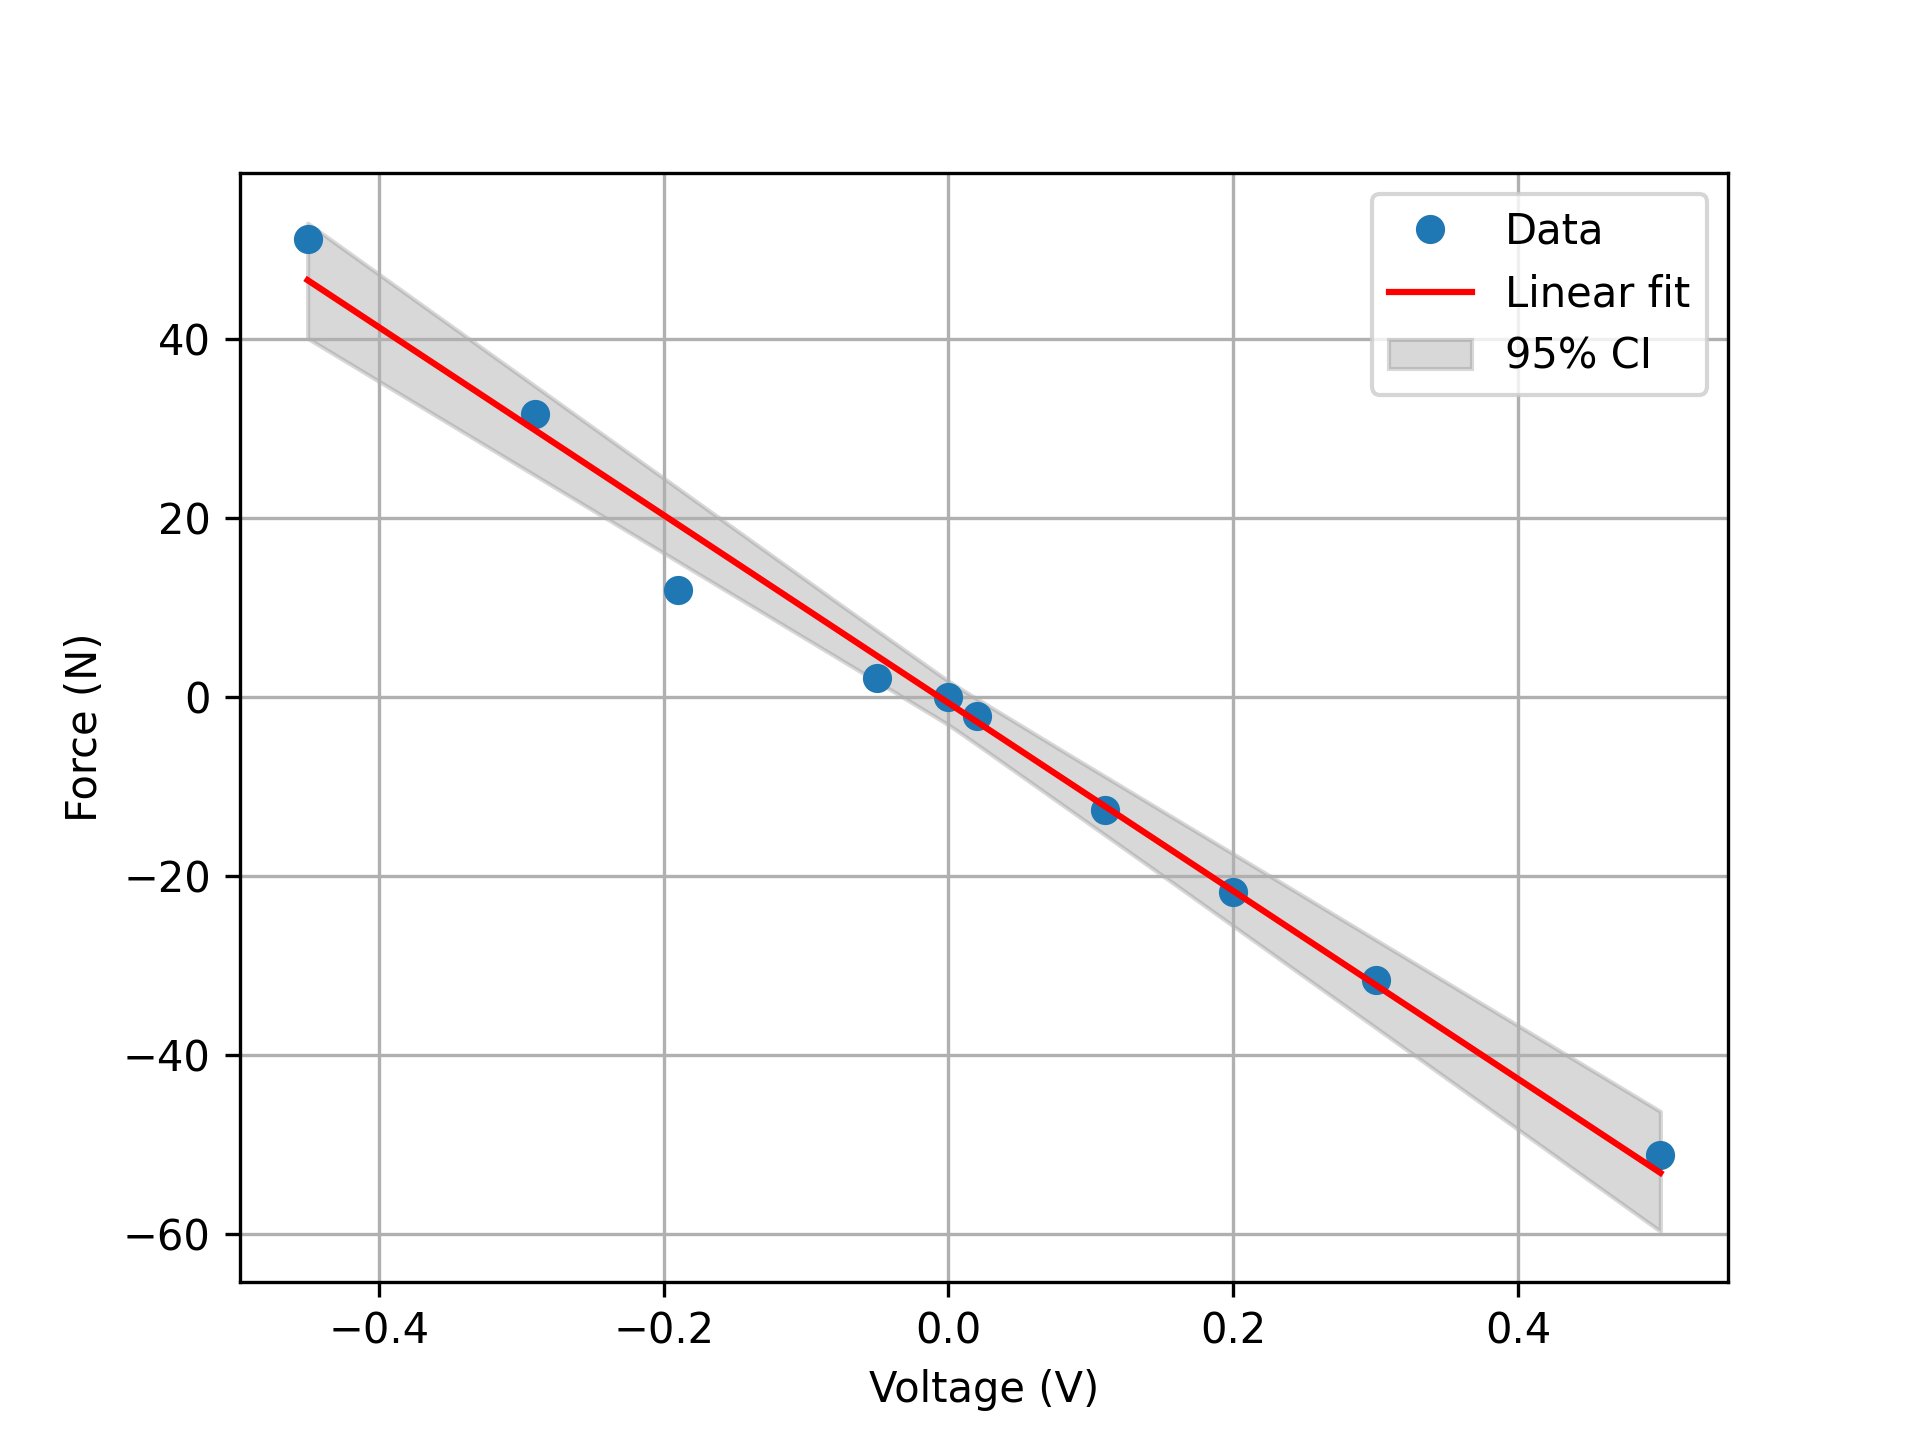
\includegraphics[width=0.8\textwidth]{Calibration/linearity.png}
    \caption{Lateral force transducer voltage calibration.}
    \label{fig:force_linearity}
\end{figure}

\begin{center}
    \textbf{Comment on the accuracy and linearity of the side force transducer}
\end{center}

The side force transducer consists of strain gauages in a Wheatstone bridge.
It is assumed that the location of strain gauges and the bridge configuration is setup to only measure the side force and not be affected by transverse forces.
This was not verified in the experiment as calibation was only done by applying known side forces.

The calibation line in figure \ref{fig:force_linearity} shows a strong linear relationship in the range of forces considered with an $r$ value of -0.9944.
The 95\% confidence interval for the linear fit is shown in the shaded region of the figure.
The uncertainty in forces is negligible and for voltage collected at 2 d.p. $\pm 0.005 V$ is also small.
This indicates both good accuracy and linearity of the transducer.

\subsection{\textbf{Effect Of Speed On Side Force}}

\begin{figure}[H]
    \centering
    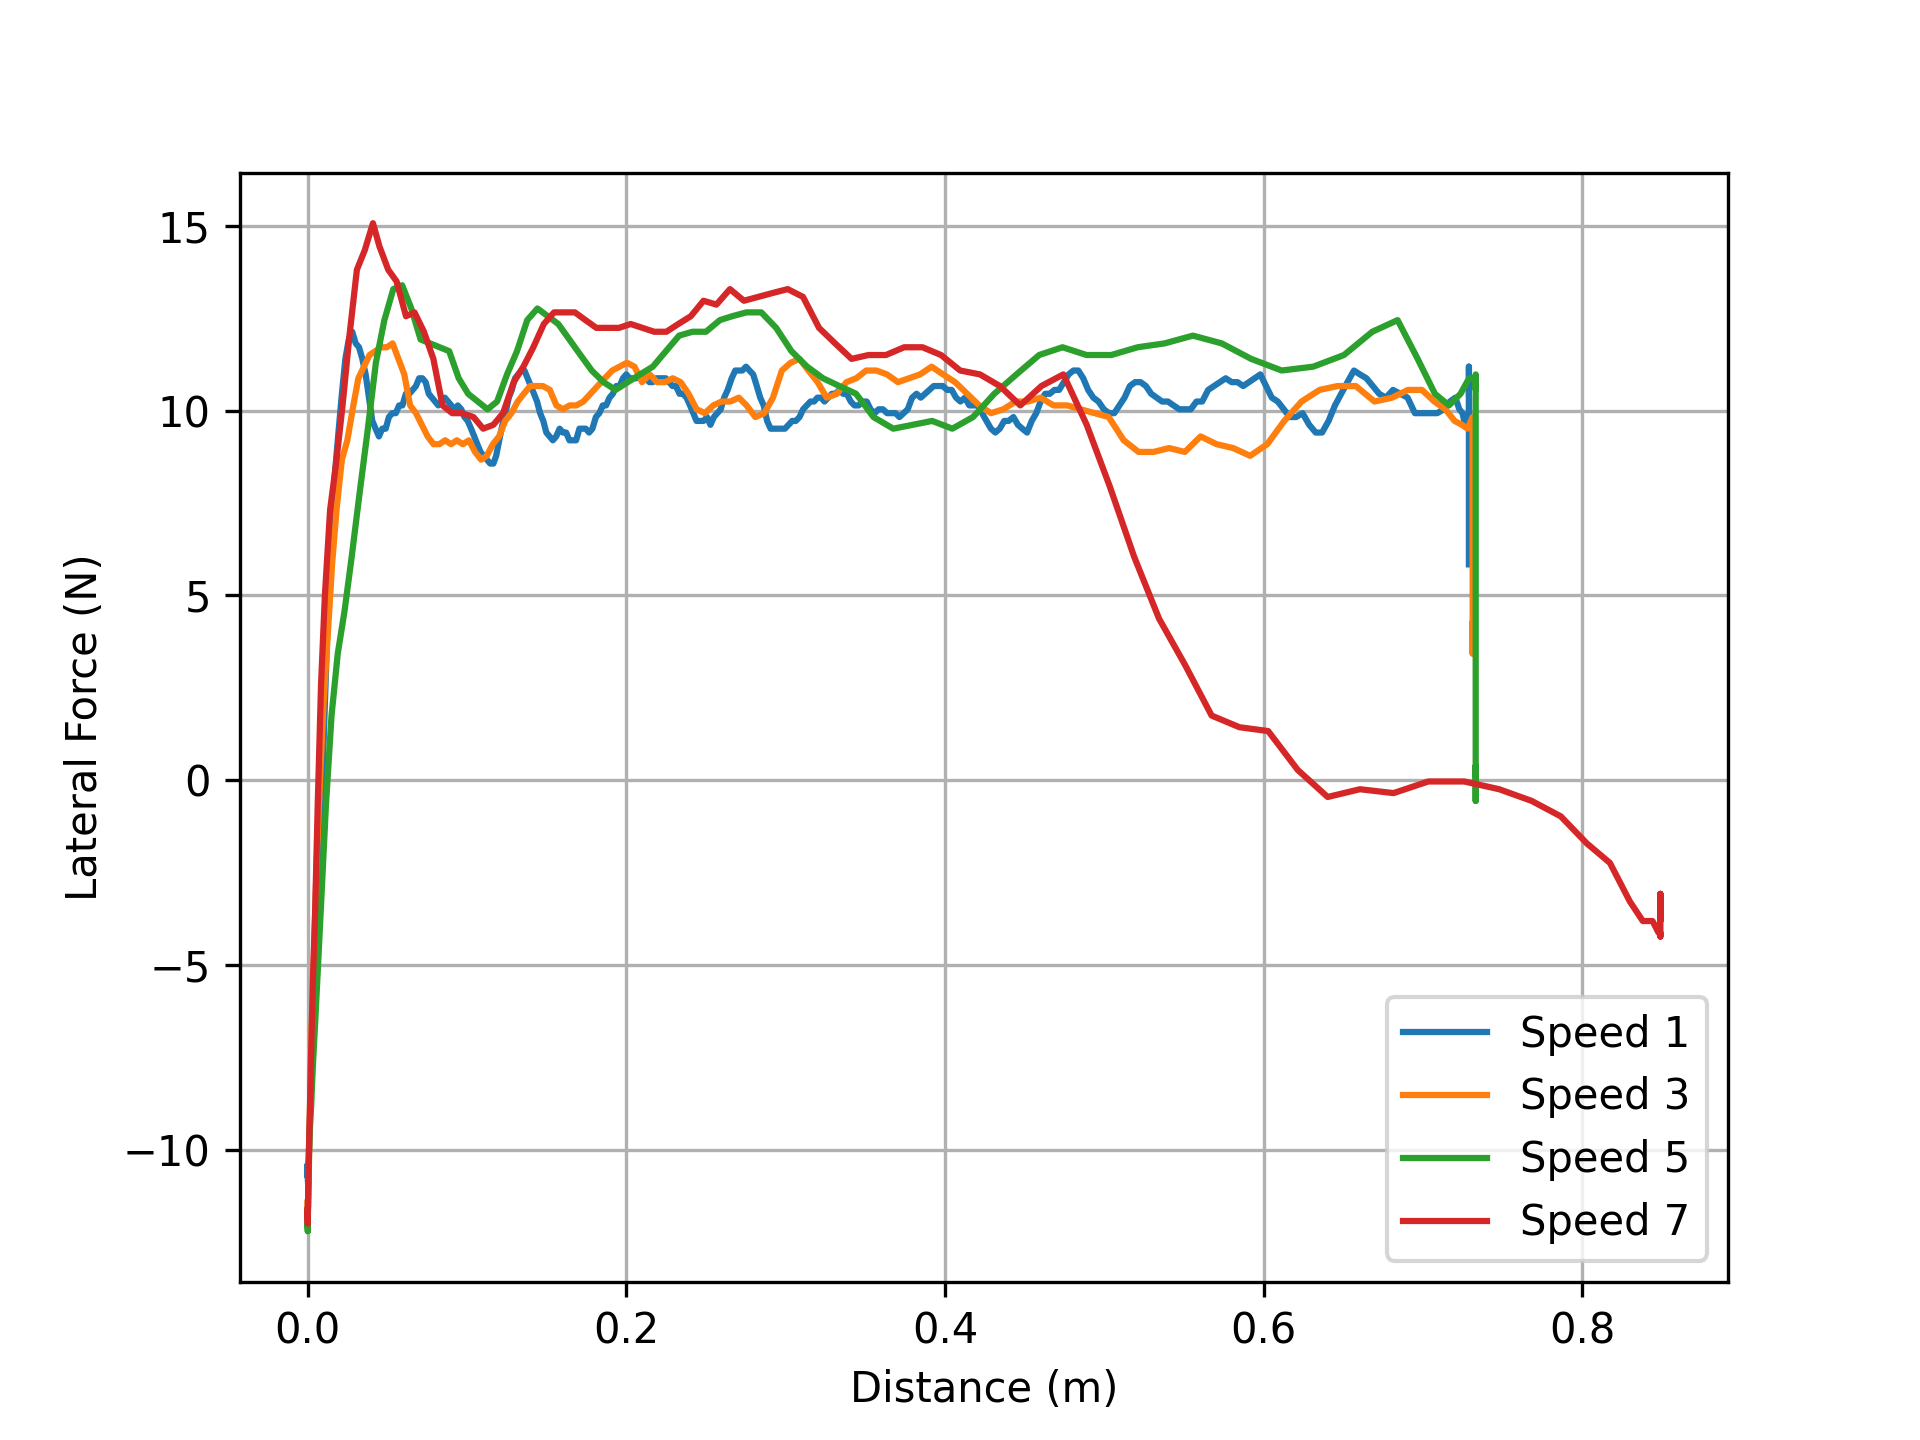
\includegraphics[width=0.8\textwidth]{4.2/force_distances.png}
    \caption{Lateral force vs. distance at $\delta = 5^\circ$ for different rolling speeds.}
    \label{fig:lateral_force_distance_speed}
\end{figure}

\begin{center}
    \textbf{Comment on the influence of rolling speed on the average steady state lateral forces
    developed by the model tyre.}
\end{center}

\subsection{\textbf{Effect of Normal Load on Steady State Side Force}}

\begin{figure}[H]
    \centering
    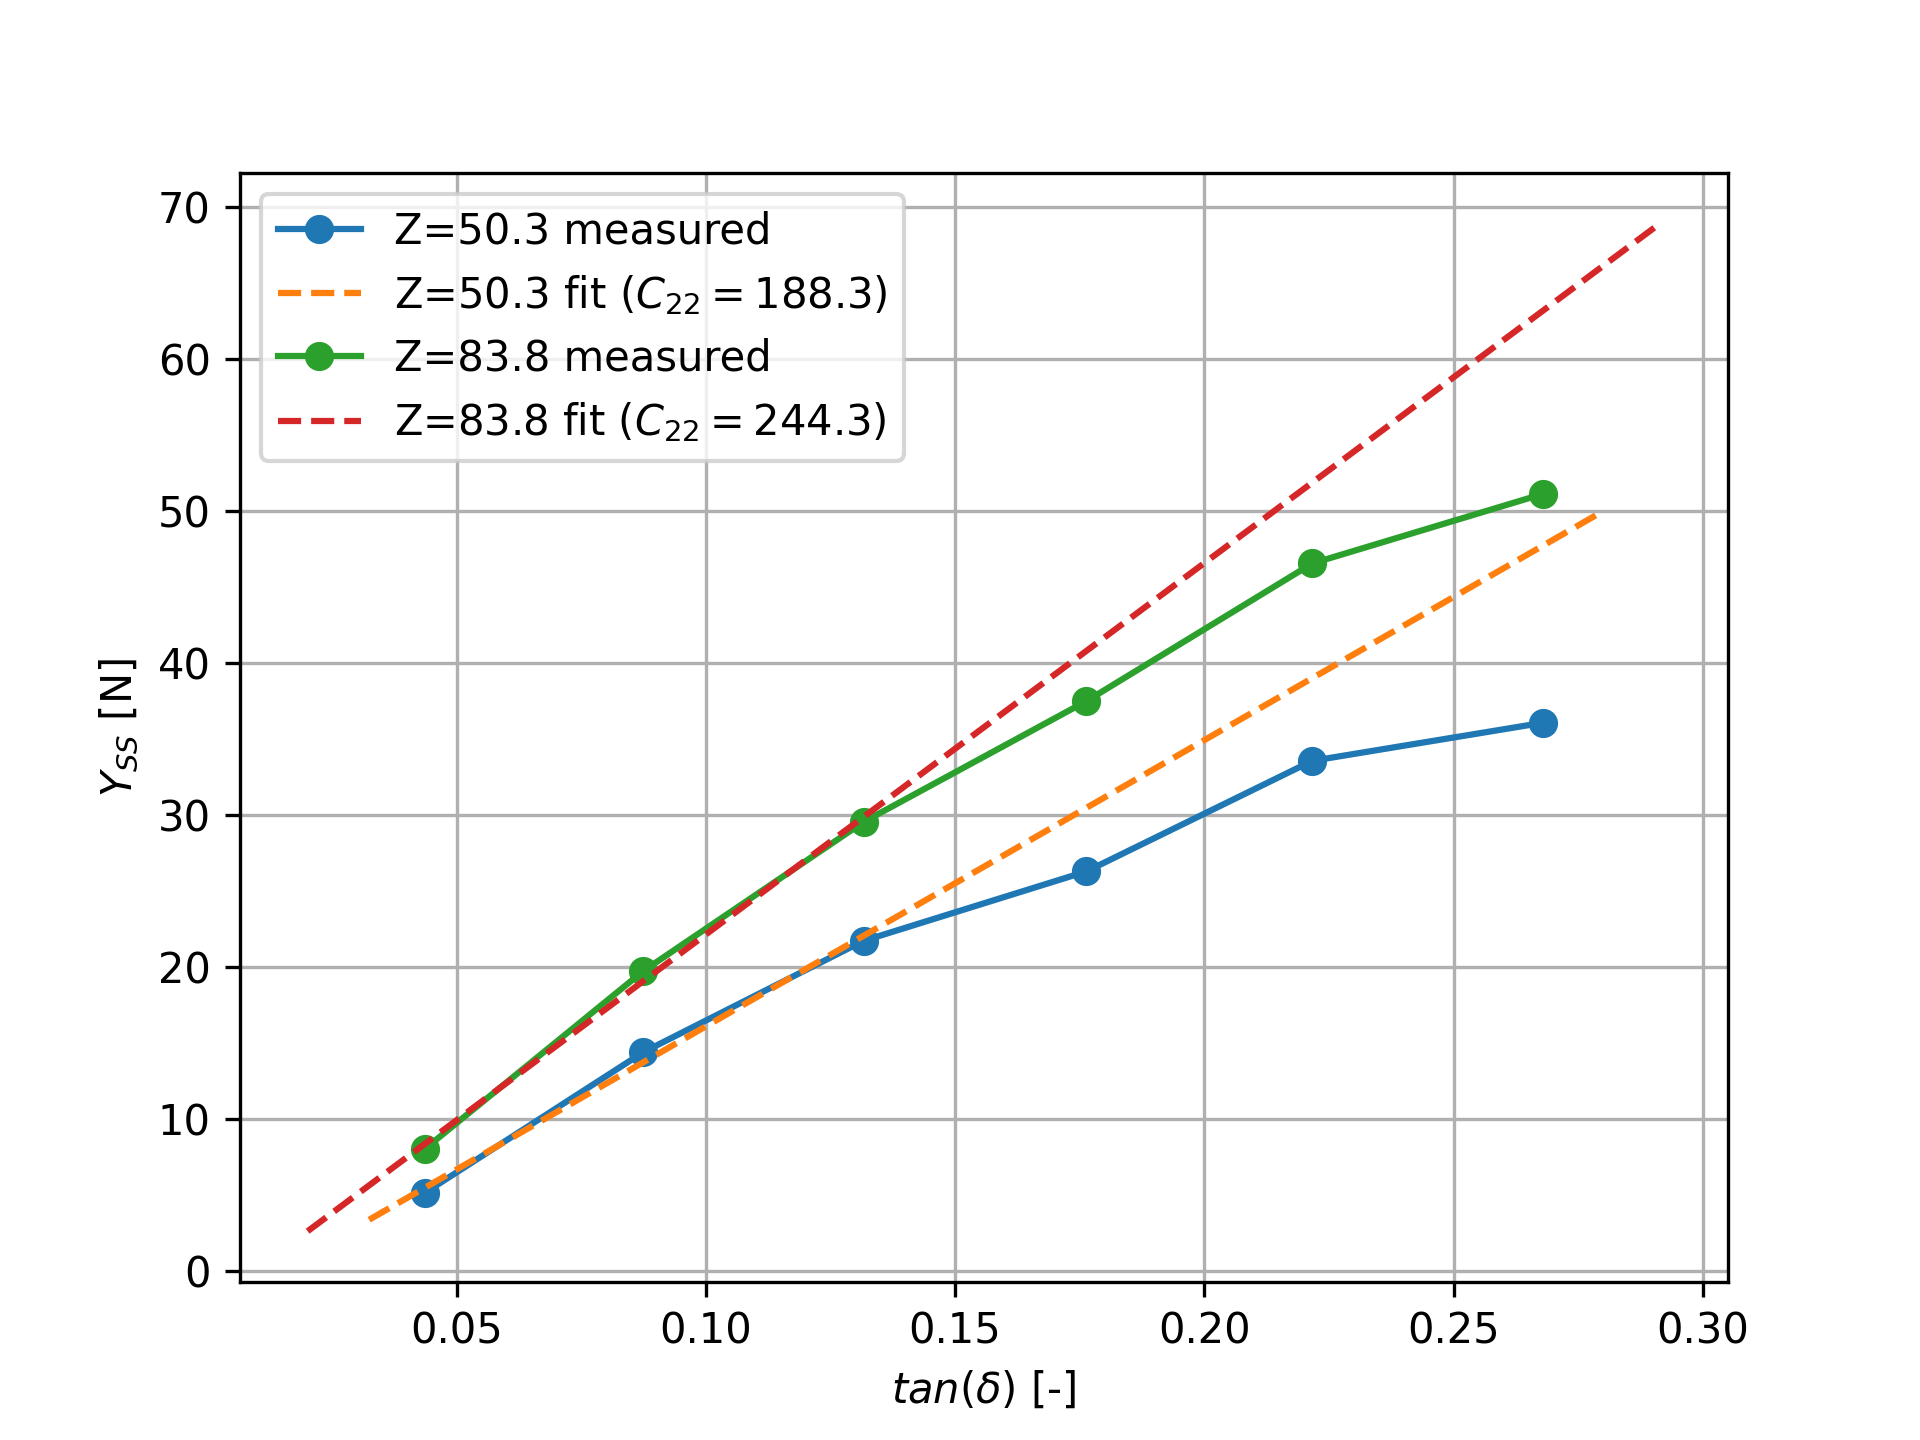
\includegraphics[width=0.8\textwidth]{4.3/Yss_vs_tandelta.png}
    \caption{Lateral force vs. tangent of steer angle.}
    \label{fig:lateral_force_distance_speed}
\end{figure}

\begin{center}
    \textbf{What causes the microslip?}
\end{center}

\begin{center}
    \textbf{Comment on the relationship between the amount of microslip in the contact area and
    the shape of the Y vs. $ \alpha $ graph}
\end{center}

\begin{center}
    \textbf{At which normal load is the tyre nearest to sliding for large
    $ \alpha $ ? Why? How is the
    linear range of Y vs.
    $ \alpha $ affected by the normal load?}
\end{center}

\section{LONGITUDINAL CREEP}

\subsection{\textbf{No Load Creep}}

\subsection{\textbf{Creep with an Applied Torque}}

\begin{center}
    \textbf{ Comment on the longitudinal deformation and compare it with the lateral deformation
    in section 4.3. Where is sliding most likely to occur? Comment also on the
    relationship between the amount of sliding in the contact area and the shape of the X
    vs.
    ξ graph.}
\end{center}



\begin{equation}
    \xi = \frac{\Delta x}{x} 
     = \frac{x_{2} - x_{1}}
            {\bigl(x_{\max} - x_{1}\bigr) + \bigl(x_{\max} - x_{2}\bigr)}.
\end{equation}

\subsection{\textbf{Combined Lateral and Longitudinal Creep}}

\begin{figure}[H]
    \centering
    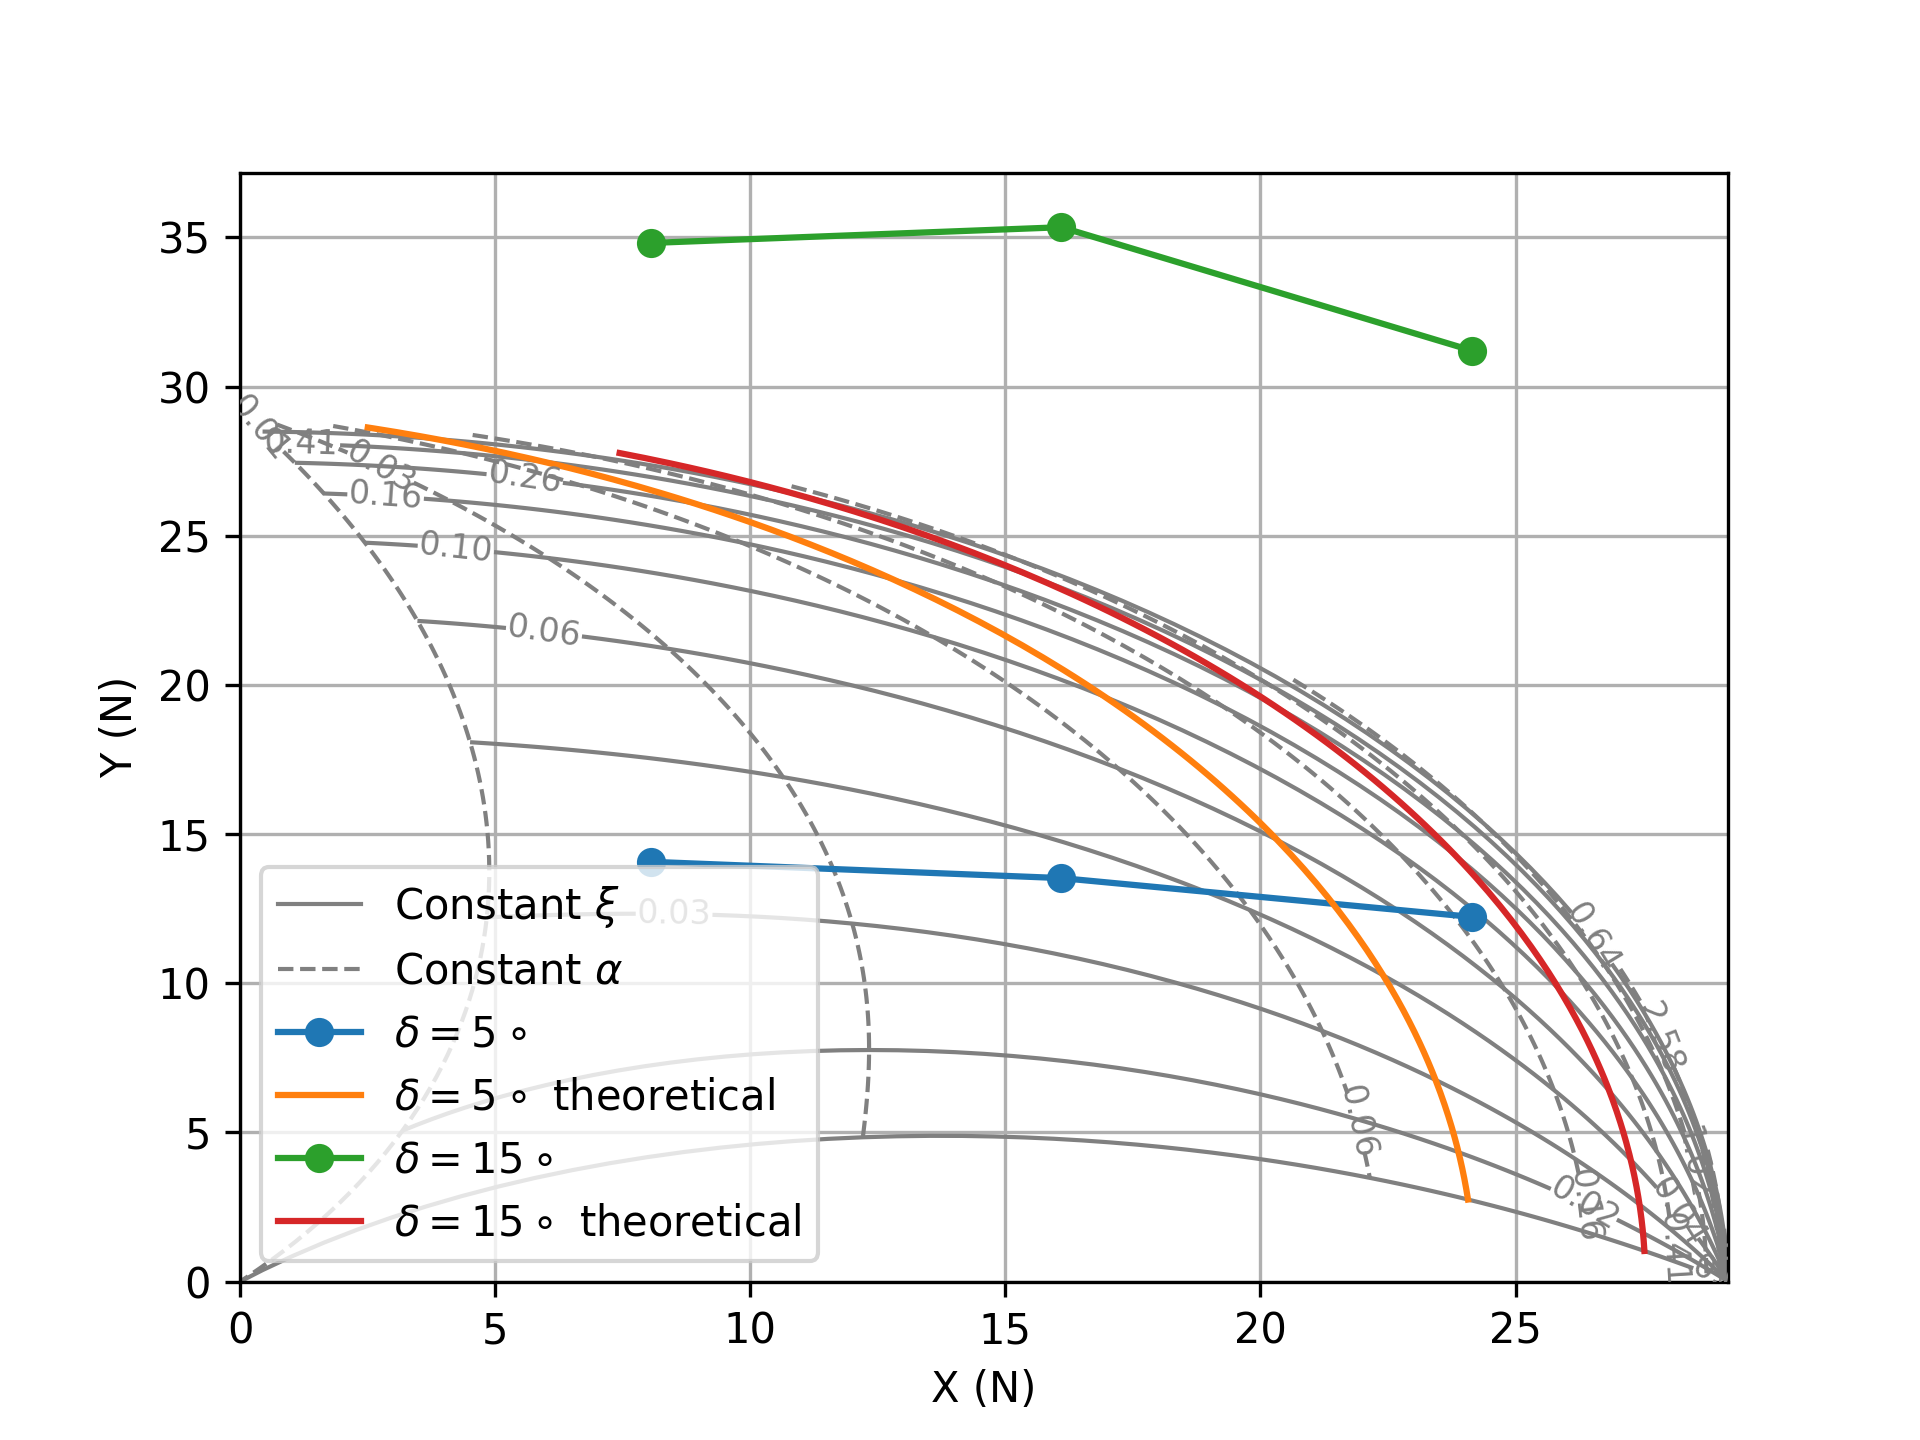
\includegraphics[width=0.8\textwidth]{5.3/XvsY.png}
    \caption{}
    \label{fig:lateral_force_vs_longitudinal_force}
\end{figure}

\begin{center}
    \textbf{Comment on the comparison between theory and experiment.}
\end{center}

\section{Appendix}

\begin{thebibliography}{9}


  \bibitem{handout}
  J. V. Taylor
  \emph{Turbine Cascade Aerodynamics Handout}
  University of Cambridge,
  October 2024.

  \bibitem{losses}
  J. D. Denton (1993).
  \emph{Loss Mechanisms in Turbomachines}
  May, 1993 

  \bibitem{fluidmech}
  S. L. Dixon
  \emph{Fluid Mechanics, Thermodynamics of Turbomachinery, FOURTH EDITION}
  1998

  \bibitem{separation}
  John M. Russell
  \emph{LENGTH AND BURSTING OF SEPARATION BUBBLES: A PHYSICAL INTERPRETATION}
  1979
\end{thebibliography}

\end{document}